\documentclass[11pt]{article}
\pagestyle{plain} 
\usepackage[text={6.5in,9.5in},centering]{geometry}
\usepackage{amsmath}
\usepackage{graphicx}
\usepackage{caption}
\usepackage{float}


%%%%%%%%%%%%%%%%%%%%%%%%%%%%%%%%%%%%%%%%%%%%%%%%%%%%%%%%%%%%%%%%%%%%%%%
% Don't touch anything above here!
%%%%%%%%%%%%%%%%%%%%%%%%%%%%%%%%%%%%%%%%%%%%%%%%%%%%%%%%%%%%%%%%%%%%%%%

\begin{document}


%%%%%%%%%%%%%%%%%%%%%%%%%%%%%%%%%%%%%%%%%%%%%%%%%%%%%%%%%%%%%%%%%%%%%%%
% Fill in your name, make sure the rest is correct
%%%%%%%%%%%%%%%%%%%%%%%%%%%%%%%%%%%%%%%%%%%%%%%%%%%%%%%%%%%%%%%%%%%%%%%
\noindent Your name \\
Math 87 HW 1 \\
Due 2/02/22 

\hrulefill



%This is how you make a list....
\begin{enumerate}


%%%%%%%%%%%%%%%%%%%%%%%%%%%%%%%%%%%%%%%%%%%%%%%%%%%%%%%%%%%%%%%%%%%%%%%
% Problem 1
%%%%%%%%%%%%%%%%%%%%%%%%%%%%%%%%%%%%%%%%%%%%%%%%%%%%%%%%%%%%%%%%%%%%%%%


\item 
\begin{enumerate}
\item Fill in your answers here. This is how you type things in-line in math mode, $y = f(x)$.


\item Here's how you make an equation:
	\begin{equation*}
	\frac{dy}{dx} = \sin(x) x^2 
	\end{equation*}


\item You can align multiple lines of math like this:

	\begin{align*}
	f(x) &= x^3 - 4x^2 + 3x - 12 \\
		&= x^2(x - 4) + 3(x-4) \\
		&= (x^2 + 3)(x-4)
	\end{align*}  


\end{enumerate}


%%%%%%%%%%%%%%%%%%%%%%%%%%%%%%%%%%%%%%%%%%%%%%%%%%%%%%%%%%%%%%%%%%%%%%%
% Problem 2
%%%%%%%%%%%%%%%%%%%%%%%%%%%%%%%%%%%%%%%%%%%%%%%%%%%%%%%%%%%%%%%%%%%%%%%

\item  
\begin{enumerate} 
\item 
\item  Here's how you make a table to report your results \\

	\begin{table}[H]
	\begin{center}
	\begin{tabular}{|c|c|c|}
	\hline 
	$x_0$ & iters & $x_*$ \\ 
	\hline 
	$1/2$ & • & • \\ 
	\hline 
	$2$ & • & • \\ 
	\hline 
	$10$ & • & • \\ 
	\hline 
	$-1/2$ & • & • \\ 
	\hline 
	$-5$ & • & • \\ 
	\hline 
	\end{tabular} 
	\caption{Newton's Method}
	\end{center}
	\end{table}
	

	\begin{table}[H]
	\begin{center}
	\begin{tabular}{|c|c|c|}
	\hline 
	$(x_0, x_1)$ & iters & $x_*$ \\ 
	\hline 
	$(0,2)$ & • & • \\ 
	\hline 
	$(0,10)$ & • & • \\ 
	\hline 
	$(-1, 2)$ & • & • \\ 
	\hline 
	$(-5, 5)$ & • & • \\ 
	\hline 
	$(-10,2)$ & • & • \\ 
	\hline 
	\end{tabular} 
	\caption{Secant Method}
	\end{center}
	\end{table}
	
	
	
	\begin{table}[H]
	\begin{center}
	\begin{tabular}{|c|c|c|}
	\hline 
	$[x_L, x_R]$ & iters & $x_*$ \\ 
	\hline 
	$[0,2]$ & • & • \\ 
	\hline 
	$[-5,5]$ & • & • \\ 
	\hline 
	$[-10,2]$ & • & • \\ 
	\hline 
    $[-1,2]$• & • & • \\ 
	\hline 
	$[0,1]$ & • & • \\ 
	\hline 
	\end{tabular} 
	\caption{Bisection Method}
	\end{center}
	\end{table}



\item 
\item Here's how you add an image to your homework: (don't forget to put axis labels and a title on your plot) \\

\begin{figure}[H]
\begin{center}
%change the file name to your file and change the scale number to make it the right size
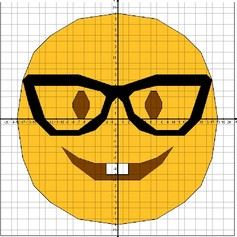
\includegraphics[scale=3]{test}
\end{center}
\caption{Math is fun!}
\end{figure}

This is how you do limits: 
\begin{equation*}
\lim_{x \to - \infty} f(x) = ???
\end{equation*}

\item 
\end{enumerate}


\end{enumerate}
\end{document} 
